
\section{Discursos de odio}


El discurso discriminatorio puede describirse como aquel discurso en clave de intenso aborrecimiento, denigración y enemistad que ataca a un individuo o un grupo de individuos por poseer --o aparentar poseer-- cierta característica protegida por tratados internacionales como el sexo, el género, la etnia, etc. Si bien no hay un consenso generalizado sobre qué configura exactamente lenguaje de odio o discriminación \cite{article192015}, un posible punto de contacto entre las distintas definiciones apuntan hacia un discurso que tienda a generar un ambiente de hostilidad contra grupos con alguna característica de las mencionadas.

En los últimos años, este tipo de discurso ha tomado gran relevancia en redes sociales y otros medios virtuales debido a su intensidad y a su relación con actos violentos contra miembros de estos grupos. A raíz de esto, estados y organizaciones supranacionales como la Unión Europea han sancionado legislación que insta a las empresas de redes sociales a moderar y eliminar contenido discriminatorio, con particular foco de aquel que insta a la violencia física.

Debido a la enorme cantidad de contenido generado por usuarios en las redes sociales, es necesario contar con cierta automatización en esta tarea bien para su análisis o para su moderación. Desde el procesamiento de lenguaje natural, la detección de discriminación puede entenderse como una clasificación de texto: dado un texto generado por un usuario, predecir si es o no contenido discriminatorio. Así mismo, puede ser de interés predecir otras características: por ejemplo, si el texto contiene un llamado a la acción violenta, si está dirigido contra un individuo o un grupo, el tipo de característica ofendida, entre otras.

Una de las limitaciones de los enfoques actuales para la detección del lenguaje discriminatorio es la falta de contexto en el mensaje. La mayoría de los estudios y recursos están hechos sobre datos fuera de contexto; es decir, mensajes aislados sin ningún tipo de contexto conversacional o del tema del cual se habla. Esto restringe la información disponible --tanto para un humano como para un sistema-- para poder discernir si un texto social es discriminatorio. Otra información usualmente faltante es la característica atacada: es común que los datasets estén anotados de manera poco granular, no brindando información acerca de si la agresión es por motivos de sexo, género, clase social, etc. Por último, una limitación puntual del español es la poca disponibilidad de recursos para esta tarea. Más aún, los datasets suelen estar anotados por anotadores que no son hablantes de las variedades dialectales de los textos utilizados, lo cual genera un déficit en su calidad al ser el lenguaje discriminatorio altamente dependiente de la jerga específica de cada región.


%En esta tesis pretendemos abordar algunas de las limitaciones marcadas. Por un lado, analizamos el impacto de agregar contexto a la detección de lenguaje discriminatorio en redes sociales. Para ello, construimos un dataset de tweets en base a las respuestas de los usuarios a los posteos de medios periodísticos en Twitter. Esto nos permite obtener dos tipos de contextos: uno “conversacional” al tener una respuesta a un tweet anterior, y uno más extenso al obtener el texto de la noticia en cuestión. El corpus fue recolectado sobre noticias relacionadas a la pandemia del COVID-19, en idioma español mayormente en su variedad dialectal rioplatense y anotado por hablantes nativos de ese dialecto con un modelo de etiquetado granular respecto a las características ofendidas.

%Sobre los comentarios de este dataset realizamos experimentos de detección de discurso de odio planteando dos tareas: detección “plana” del lenguaje discriminatorio, donde sólo predecimos una etiqueta binaria indicando presencia de lenguaje discriminatorio; y detección “granular”, donde predecimos las características ofendidas. Usando técnicas del estado del arte, obtuvimos mejoras significativas en ambas tareas al agregar contexto como entrada de cada instancia, tanto en su forma corta (sólo el titular/tweet de la noticia) como en su forma larga (titular + cuerpo de la noticia). Así mismo, observamos que un clasificador entrenado para la tarea “granular” mejora levemente su performance al ser evaluado para la tarea “plana”, obviando los posibles errores de motivos discriminatorios. Combinando la adición de contexto y granularidad, un clasificador para la detección de lenguaje discriminatorio obtiene mejoras considerables sobre un BERT en español que sólo consume el texto del comentario.

Considerando la detección de discurso de odio dentro del área más abarcativa de clasificación de documentos en dominios sociales, analizamos algunos aspectos generales para tareas relacionadas como el análisis de sentimiento y la detección de emociones, entre otras. En particular, analizamos el desempeño de las técnicas de representación al ser entrenadas en distintos dominios. En general, los modelos de representación son entrenados a partir de textos de dominios “formales”, como pueden ser Wikipedia u otras fuentes similares. En esta tesis analizamos el efecto de generar estas representaciones desde textos informales. Observamos que –desde los word embeddings hasta los modelos pre-entrenados basados en transformers– las representaciones generadas son robustas y mejoran la performance en un conjunto de tareas de clasificación en textos sociales. Sobre los modelos pre-entrenados, estudiamos el impacto de entrenarlos desde cero en textos sociales o efectuar una adaptación sobre este dominio

Todos los estudios y recursos de esta tesis fueron realizados en español. Como un objetivo secundario, pretendemos mitigar la enorme asimetría de recursos existente en el área del procesamiento del lenguaje natural.


\section{Algunos casos resonantes}

Para poner en contexto la necesidad de desarrollar herramientas que puedan ayudar a la detección de este fenómeno, comentamos algunos casos puntuales que han tenido lugar en los últimos años y en los cuales se ha estudiado la incidencia de la diseminación de discurso de odio --mayormente racista o xenófobo-- en redes sociales. Si bien nos centraremos en los casos más resonantes, donde este fenómeno haya co-ocurrido con algún evento violento en la vida real, la exposición a este discurso en medios virtuales tiene impactos negativos en la psiquis de sus objetivos \cite{saha2019prevalence} y prepara un terreno hostil y de deshumanización contra un grupo vulnerado, como inmigrantes, minorías religiosas y sexuales \cite{bilewicz2020hate}, algo que ya ha sido estudiado a lo largo de décadas.


\subsection{Atentados en Charlottesville}

En Agosto del 2017, una gran movilización organizada por varios movimientos de ultraderecha y supremacistas blancos tuvo lugar en la ciudad de Charlottesville, Virginia, Estados Unidos, y particularmente centrada en la Universidad de dicho Estado. Esta concentración fue llamada en el medio del intento de universitarios y el movimiento Black Lives Matter (BLM) de remover estatuas de militares conferados pro-esclavitud de la Guerra de Secesión; en el caso de la Universidad de Virginia, sobre la estatua de Robert Lee. Más aún, tuvo lugar durante los primeros meses del mandato de Donald Trump.

Numerosos grupos de ultraderecha, neonazis, neo-confederados, entre otros, convocaron a la marcha ``Unite the Right'', diseñada como una campaña militar y organizada hasta 3 meses antes de su concreción. \citet{blout2020white} describen la experiencia de Charlottesville como la de un ``terrorismo inmersivo'', ya que generaron un ámbito de terror en varios ``teatros'' (como lo llaman los autores, usando jerga militar). Principalmente, el teatro físico, con la marcha y enfrentamientos con las contra-movilizaciones, la intimidante marcha de antorchas, y el asesinato de Heather Heyer atropellada por un manifestante neo-nazi. Así mismo, el teatro ``virtual'', que sirvió para generar un clima de intimidación en la previa, durante, y luego del evento. En el trabajo mencionado, se cita particularmente una campaña judeófoba contra el alcalde de Charlottesville (de ascendencia judía) y el vicemayor (afroamericano).

Los autores llegan a la conclusión de que el evento fue organizado de manera centralizada, tanto en su planificación como despliegue en un intento de ejercicio militar. También concluyen que, la propaganda y la información propagada por los organizadores sirvió para publicitar y reclutar a simpatizantes y también para aterrorizar a la población. Esta propaganda tuvo lugar tanto en medios impresos (por ejemplo, posters pegados en las calles) como por medios virtuales y redes sociales como Facebook, Twitter o Discord. \citet{klein2019twitter} analiza los intercambios en Twitter entre los dos bandos (manifestantes de ultraderecha y los contramanifestantes) y muestra que, en el caso de quienes se encontraban del lado de la marcha de UtR, se identifica como enemigos a los musulmanes, liberales o izquierdistas,a miembros de la comunidad LGBTQ, judíos, entre otros.


\subsection{Matanza en Sinagoga de Pittsburgh}


\begin{figure}[t]
    \centering
    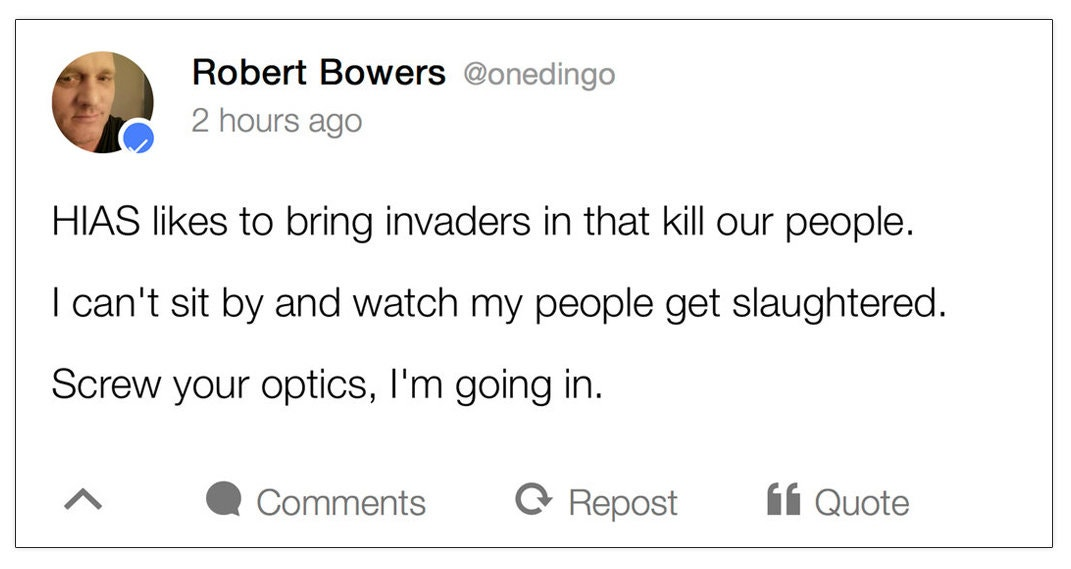
\includegraphics[height=6cm, keepaspectratio]{img/gab-pittsburgh-post.jpg}
    \caption{Último post de Robert Bowers, tirador en la masacre de Pittsburgh, en la red social Gab.}
    \label{fig:gab_post}
\end{figure}


En Octubre de 2018, un hombre fuertemente armado entró a la sinagoga ``El Árbol de la Vida'' en Pittsburgh, Pensilvania, Estados Unidos. Luego de gritar ``muerte a los judíos'', abrió fuego contra la multitud matando 11 personas y dejando decenas de heridos, la más grande matanza de judíos en EEUU de la que se tenga registro.

El tirador, Richard Bowers, era usuario activo de Gab \footnote{\url{https://gab.com/}}. Gab es una red social que nació en 2016 bajo la égida de la defensa de la ``libertad de expresión'' a raíz de la creciente moderación de Twitter a discursos discriminatorios. Desde entonces, ha sido el refugio de activistas de la derecha alternativa, supremacistas raciales, grupos conspiracionistas y otros elementos reaccionarios. El asesino en cuestión posteaba frecuentemente contenido antisemita en dicha red social \cite{mcilroy2019welcome}. En su último post en dicha red social, horas antes de la masacre, Bowers posteó una amenaza diciendo que no podía tolerar ver a su gente ser asesinada (por judíos).

A raíz de esto, Gab --descrita como el ``Twitter racista''-- fue dado de baja durante cierto tiempo al serle negado alojamiento web. Desde entonces, diversos trabajos han estudiado y recopilado el contenido discriminatorio en esta red social \cite{mcilroy2019welcome,kennedy2018gab} como material de estudio.



\subsection{Masacre Rohingya en Myanmar}m
% https://www.quigsclass.com/uploads/7/2/6/8/72681355/5_myanmar_facebook.pdf
%
Entre 2016 y 2017, una matanza de la etnia Rohingya, un grupo étnico musulmán, tuvo lugar en la República de Myanmar (ex Birmania). Cerca de 25 mil personas fueron masacradas y un éxodo de más de 700 mil personas tuvo lugar hacia la lindante Bangladesh, conformando el campamento de refugiados más grande del mundo. La ONU y algunos estados nacionales han calificado lo ocurrido como un ``genocidio''.


Si bien el sometimiento de este pueblo tiene lugar hace décadas, en los últimos años tuvo un gran recrudecimiento motorizado desde altas esferas militares. En ese punto, las redes sociales han jugado un rol de difusor y catalizador de incitaciones a la violencia y noticias falsas alrededor de esta población marginada. Según un informe solicitado por Facebook acerca de la situación en Myanmar \cite{warofka2018independent}, gran parte de este problema se debe a un déficit en el ``alfabetismo digital''(sic) de la población de Myanmar, que usa casi exclusivamente Internet a través de dicha red social. Enviados de las Naciones Unidas han acusado directamente a Facebook de haber servido como intermediario de discurso de odio a través de su plataforma \footnote{\url{https://www.reuters.com/article/us-myanmar-rohingya-facebook/u-n-investigators-cite-facebook-role-in-myanmar-crisis-idUKKCN1GO2PN}}.

Grupos de derechos humanos de ese país han instado a Facebook a invertir recursos en el control del discurso de odio, particularmente aquel que insta a la violencia física \cite{irrawaddy2018zuckerberg}. A finales de 2021, un grupo de refugiados rohingya denunció a Facebook por 150 mil millones de dólares \footnote{\url{https://www.bbc.com/news/world-asia-59558090}} por haber promovido la violencia contra este grupo, luego de haber admitido en 2018 que no hizo lo suficiente para detener la proliferación del discurso de odio en dicha red social.

Este hecho cuenta con una particularidad: apunta a un idioma --el birmano, idioma oficial en Myanmar-- que dispone de pocos recursos en el área del Procesamiento del Lenguaje Natural. La inmensa mayoría de los recursos y estudios están dedicados al idioma inglés, ignorando las particularidades de cada idioma y el componente cultural de algunas tareas, como en este caso la detección de discurso de odio. Según Reuters, para finales de 2018, Facebook no contaba con ningún empleado en Myanmar \footnote{\url{https://www.reuters.com/investigates/special-report/myanmar-facebook-hate/}} ni tampoco quedaba claro que alguno de sus empleados dedicados a la tarea del monitoreo hablase birmano.





\section{Avances en IA y NLP}

En los últimos 10 años, el área en general de la Inteligencia Artificial ha sido sacudida por la irrupción de las redes neuronales en el centro de la escena. Desde la disciplina de Visión por Computadora, la conjunción de datasets de gran tamaño como ImageNet \cite{imagenet2009deng} y la utilización de dispositivos de gran poder de cómputo como las GPUs, además del desarrollo de mejores algoritmos (como la utilización de distintas funciones de activación) posibilitaron que las redes neuronales obtengan mejoras considerables en el desempeño de tareas de reconocimiento de imágenes. \todo{agregar citas}

Este boom inicial en el área de CV tuvo su primera repercusión cerca del año 2013, con el desarrollo de los word-embeddings. La técnica de \emph{word2vec}\cite{mikolov2013distributed} permitió generar representaciones de palabras de manera eficiente sobre grandes cantidades de datos no etiquetados. Estas representaciones de cada palabra (podemos pensarlas como vectores de largo fijo asignadas a cada token) han sido la ``salsa secreta'' que permitió el éxito de las redes neuronales en NLP, permitiendo una mejora en las tareas de reconocimiento de entidades nombradas (NER), POS tagging, parsing, clasificación de textos, entre otras. Otro componente de este éxito de las redes neuronales ha sido el uso de redes recurrentes como las Long Short-Term memory (LSTM) \cite{hochreiter1997long} o las Gated Recurrent Units (GRU) \cite{cho-etal-2014-learning}, que codifican las representaciones de una manera autorregresiva.

Un caso de éxito particular ha sido el de la traducción automática. La arquitectura sequence-to-sequence (seq2seq) \cite{sutskever2014sequence} permitió que una red neuronal compuesta de un codificador y un decodificador pudiera traducir una secuencia de tokens a otra secuencia de tokens, mejorando el desempeño de tareas de traducción automática. Más aún, permitiendo reemplazar sistemas realmente complejos de Statistical Machine Translations (SMT) por sistemas más simples y con mucha mejor performance.

Las arquitecturas recurrentes, sin embargo, adolecen algunos problemas. En primer lugar, su caracter autorregresivo inhibe la paralelización: necesitamos primero calcular el paso anterior para poder computar el siguiente. Otro problema a mencionar es que sufren de \emph{locality bias}: tienden a favorecer relaciones con entidades cercanas del texto debido a su estructura Markoviana. Estas dos cuestiones, por un lado, ponen cierta cota a la performance en algunas tareas, y por otro, hacen complejo el entrenamiento de redes neuronales verdaderamente profundas, como son utilizadas en el campo de Computer Vision. A su vez, otra limitación del enfoque de utilización de redes neuronales + embeddings es que reutilizamos muy poco entre problemas: sólo la capa de embeddings, el resto debe ser re-entrenado.

En 2017, \citet{vaswani2017attention} propusieron una arquitectura que elimina la estructura recurrente: los \emph{Transformers}. Este modelo utiliza únicamente múltiples capas de auto-atención para el problema de traducción, pudiendo superar el estado del arte y con un entrenamiento más eficiente.

Utilizando esta arquitectura, GPT y BERT
\footnote{Ver las slides de Jacob Devlin, uno de los creadores de BERT acerca de los problemas de las RNN\url{https://nlp.stanford.edu/seminar/details/jdevlin.pdf}} supusieron un cambio rotundo en el modo en que hacemos NLP hoy día: en lugar de entrenar una red neuronal casi desde cero (quizás sólo con una capa de embeddings con pesos iniciales pre-calculados) sólo ajustamos (\emph{fine-tune}) una gran red neuronal pre-entrenada sobre un dataset de entrenamiento. Estos modelos supusieron un breakthrough en el área de NLP, mejorando la performance sensiblemente en benchmarks de tareas como GLUE.

Estos avances han permitido atacar numerosas tareas que quizás parecían fuera de alcance para el área de NLP o bien tenían performances muy decepcionantes. Entre ellas, la detección de discurso de odio.

\subsection{Asimetría de recursos}

Como dice la ``Regla de Bender''\cite{bender2011achieving}

\begin{quote}
    Do state the name of the language that is being studied, even if it's English. Acknowledging that we are working on a particular language foregrounds the possibility that the techniques may in fact be language specific. Conversely, neglecting to state that the particular data used were in, say, English, gives [a] false veneer of language-independence to the work.
\end{quote}

Este punto es importante ya que, a pesar de ser el segundo idioma en hablantes nativos (por delante del inglés), los recursos suelen ser escasos y siempre a la rastra y reproducción de resultados en inglés. \todo{quizás esto lo mandaríamos a otro lado}



\section{Aportes de este trabajo}

En esta tesis nos proponemos hacer un aporte en el sentido de desarrollar mejores mecanismos automáticos de detección de discurso de odio. Si bien el área de NLP ha avanzado enormemente en los últimos años, y esta subdisciplina en particular ha recibido numeroso interés, creemos que muchos de los enfoques actuales inhiben un avance cualitativo en la detección de este pernicioso fenómeno en medios sociales.

Para ello, en primer lugar estudiamos técnicas de detección sobre datasets ya existentes, utilizando técnicas del estado del arte. En base a la observación de algunos datasets y la literatura en general, plantearemos un nuevo problema: la detección \emph{contextualizada} de discurso de odio. Para ello, construimos un dataset de comentarios de discurso de odio sobre comentarios de redes sociales en noticias de medios gráficos argentinos, y lo etiquetamos con hablantes nativos. Este dataset es un aporte importante en sí ya que es uno de los primeros datasets que incluyen información contextual, y es el único a nuestro conocimiento en español que tiene esta información, y el primero en la variedad dialectal rioplatense. \todo{Decir algo que lo recolectamos durante la pandemia del COVID-19}

Con este dataset, exploramos la siguiente pregunta: ¿pueden los métodos actuales basados en modelos pre-entrenados aprovechar información adicional de contexto para mejorar la clasificación de discurso de odio? Este punto ha sido poco estudiado en la literatura, y consideramos que es una pregunta de interés para atravesar los límites de la clasificación basada en una única fuente de información (el comentario analizado). En base a los experimentos realizados, encontramos evidencia que el contexto puede brindar información útil para detectar este fenómeno. Particularmente, observamos que para los mensajes de odio contra ciertos grupos --por ejemplo, contra la comunidad LGBTI-- el contexto puede brindar información aún más útil para su detección.

Finalmente, realizamos un estudio más en general sobre la \emph{adaptación de dominio} en tareas de clasificación de redes sociales. Para ello, generamos un modelo de lenguaje pre-entrenado sobre textos sociales en español al que bautizamos \robertuito{}, el primero disponible y a gran escala en este idioma. Comparamos la performance de este modelo contra otros modelos pre-entrenados sobre textos formales, y contra modelos ajustados al dominio social. Esta comparación es de interés ya que el ajuste de dominio es relativamente económico frente al enorme costo de entrenamiento que tienen construir modelos como \robertuito{}. Observamos que para todas las tareas, \robertuito{} obtiene una performance del estado del arte, pero el ajuste de dominio recorta considerablemente el gap de performance contra otros modelos.

Un aporte en general de esta tesis es que todos los estudios y recursos han sido realizados en español. Vista la enorme asimetría que hay con otros idiomas, y teniendo en cuenta que el español es el segundo idioma en hablantes nativos del mundo, consideramos necesario mitigar este desbalance de recursos.